\chapter{Experiments}
\label{ch:experiments}


\section{Machine properties}
Within the experiments it was used macbook pro middle 2018 with Coffee Lake/8th generation: a 2.2GHz Core i7 processor with six cores and with intel turbo boost up to 4.1GHz.

\section{Data}
The experimental \ref{fig:ct_spine} data set was splitted into dedicated training (with ground-truth labels) and test sets each 242 and 60 scans accordingly. The scans were re-sample  at 1mm x 1mm x 1mm resolution meaning each pixel in the generated samples from the scans provided a 3 dimensional 1mm section of the patient spine.
\begin{figure}[h]
    \centering 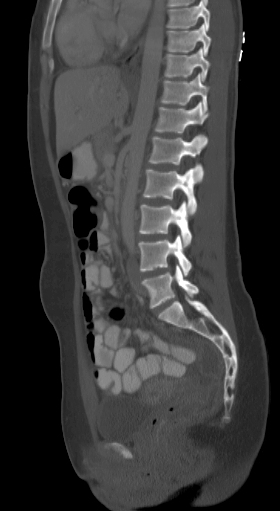
\includegraphics[width=3cm]{images/ct-spine.jpg}
    \caption {Train sample of CT spine scan}
    \label{fig:ct_spine}
\end{figure}


\section{Training models}
To recap input to detection model was initially $64x64x80$ particular scan which was transformed (5 crops) what afterwards got shape of $32x32x40$. It worth to mention, jointly training process it was applied padding which discarded the outer border of scan producing $16x16x20$ shape so far. In simplified terms, it reduced edge artifacts in the detection and led to improved mean localization scores. During roughly 17 hours the detection model had been training for 50 epochs. The validation Dice score achieved 0.911 whereas validation accuracy was 0.985. 

In regard of identification model, which was fully CNN the particular input was sized of $8x80x320$. During roughly 10 hours the identification model had been training for 35 epochs. At test time it was passed whole slices of single input scan, padded to the nearest and multiple of 16.


\section{Results}
From left to right \ref{fig:step_step_predictions} figure represents the single scan path in terms of full pipeline per each step. 

\begin{figure}[h]
    \centering 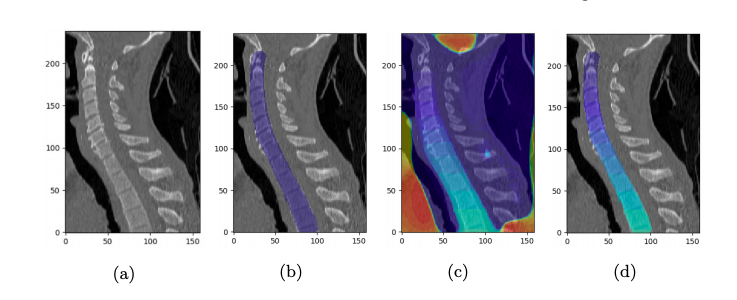
\includegraphics[width=10cm]{images/step_step_predictions.png}
    \caption {(a) shows an original scan in grey scale, (b) shows the output of the detection model applied to the scan, (c) shows the output of the identification model
    applied to the scan, (d) shows (b) and (c) multiplied together to produce a final prediction for each pixel.}
    \label{fig:step_step_predictions}
\end{figure}

As it was mentioned before the resulting measurements have been calculated within testing set of 60 scans of various patient by measured Dice score and metrics as id rate, localization error which derived into mean localization distance error and standard deviation localization distance error.

The 3 resulting random pipeline predictions can be observed at \ref{fig:predictions} figure which represents predictions themselves as well as additional impacting information as ground-truth and localization error. 
\begin{figure}[h]
    \centering 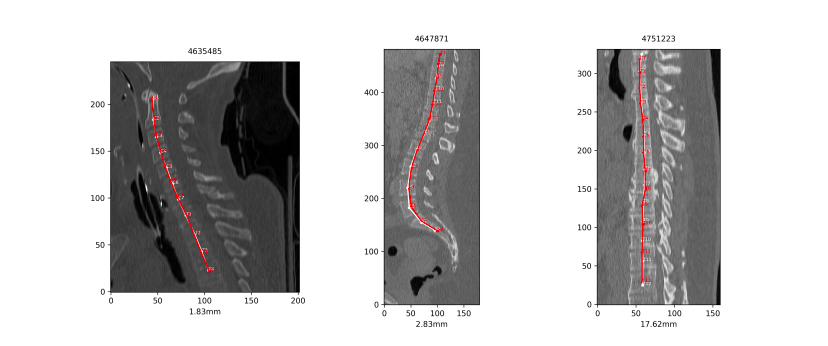
\includegraphics[width=10cm]{images/predictions.png}
    \caption {visualization of 3 random predictions, whereas the red points denote pipeline centroid predictions, the white points denote ground-truth centroid locations. On top of that each scan designated the mean localization error for particular scan.}
    \label{fig:predictions}
\end{figure}

\section{Competitors}
As the baseline comparison it was considered \cite{Liao2018} "Joint Vertebrae Identification and Localization in Spinal CT Images by Combining Short-Range and Long-Range Contextual Information" state-of-the-art work. The proposed benchmark pipeline is shown at \ref{fig:competitor} figure.

\begin{figure}[h]
    \centering 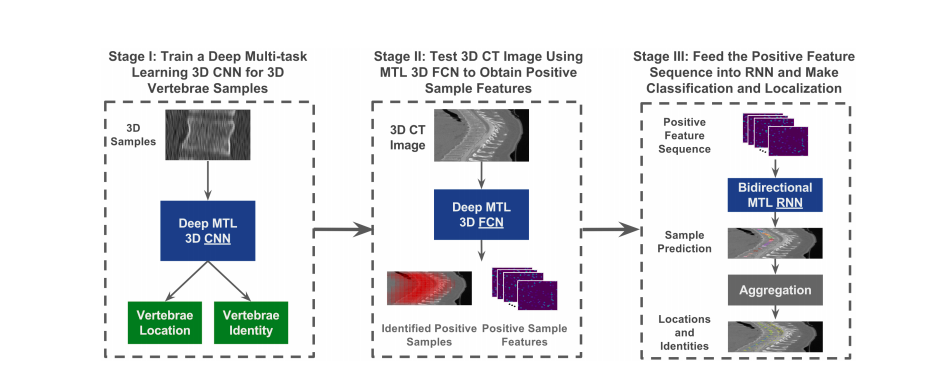
\includegraphics[width=10cm]{images/competitor.png}
    \caption {Overall architecture of the competitor proposed method for vertebrae identification and localization}
    \label{fig:competitor}
\end{figure}

The overall architecture of the proposed method may be traversed as three-stage approach. In the first stage, it was applied deep multi-task 3D CNN using randomly cropped 3D vertebrae samples. Afterwards within second stage transform trained multi-task 3D CNN into a multi-task 3D fully convolutional network by converting the fully connected layers to 3D convolutional layers. Decisively within third stage the extracted sample features will be ordered and form a set of feature sequences.


Assimilating the results the following table takes place:
